% !TEX root = slt21_lec_notes.tex
\chapter{Maximum entropy and posterior agreement}
\chaptermark{Entropy and agreement}

\section{Introduction}
\label{sec:intro}

We present here an alternative statistical learning method called ME+PA (maximum entropy + posterior agreement). This method is robust and can be applied to a wide variety of learning problems. In addition, it has been experimentally demonstrated that it generalizes better than empirical risk minimization techniques in different domains, including brain image analysis~\cite{gorbach2018pipeline, wegmayr2020entrack}, access control~\cite{frank2009probabilistic, cotrini2019next},~minimum spanning trees~\cite{gronskiy2014informative}, and predicting rankings in chess tournaments~\cite{busse2013approximate}. In particular, the notion of posterior agreement captures a notion similar to that of mutual information, when seeing learning algorithms as communication channels that use models to communicate information about an underlying phenomenon.

\section{Overview of ME+PA}
\label{sec:overview}

Before making a formal presentation, we give an intuitive overview. ME+PA consists of the following steps:

\paragraph{Step 1: Hypothesis class} Define a hypothesis class $\mathcal{C}$. This indicates the class of candidate models you want to train. Examples of hypothesis classes are the class of linear regression models, the class of classification trees, and the class of neural networks with a specific architecture.

\paragraph{Step 2: Cost function} The next step is to define a cost function $R$. This function takes as input a model $c \in \mathcal{C}$ and an observation $X$ and produces a cost value $R(c, X)$ measuring how well the model fits the given observation. Since cost functions are usually defined by humans, we require cost functions to be non-negative.

\paragraph{Step 3: Maximum entropy} For an arbitrary observation $X$, we now define a posterior probability distribution $p(\cdot \mid X)$ over $\mathcal{C}$, conditioned on $X$. For $c \in \mathcal{C}$, $p(c \mid X)$ should measure how much we believe that $c$ is the right model for $X$. This belief is quantified by $R(c, X)$. The lower this cost is, the more we believe that $c$ is the right model for $X$. We argue later in Section~\ref{sec:max_entropy} that a natural posterior distribution that fulfils this requirement is the \emph{Gibbs distribution induced by $R$}:
%
\begin{equation}
p(c \mid X) \propto \exp\left(- \frac{1}{T} R(c, X)\right).
\label{eq:max_ent_dist}
\end{equation}
%
where $T > 0$ is a hyper-parameter called the \emph{temperature}.

\paragraph{Step 4: Posterior agreement} We show in Section~\ref{sec:array} that merely picking the ``most likely'' model $c$ according to $p(c \mid X)$ amounts to overfitting and, therefore, it is not enough to generalize well. We use instead two independent observations $X'$ and $X''$ and define the \emph{posterior agreement kernel} between $X'$ and $X''$:
%
\begin{equation}
\kappa(X', X'') := \sum_{c \in C} p(c \mid X) p(c \mid X'').
\label{eq:kernel_post_agr}
\end{equation}
%
This kernel can be used to select a value for $T$ from a set of candidate temperatures $\mathcal{T}$. It can even be used to select a cost function $R$ among a set of candidate cost functions $\mathcal{R}$:
%
\begin{equation}
T^*, R^* = \argmax_{T \in \mathcal{T}, R \in \mathcal{R}} \kappa(X', X'')
\end{equation}

Finally, the two Gibbs distributions $p(\cdot \mid X')$ and $p(\cdot \mid X'')$ can be aggregated together to yield a final distribution over models
%
\begin{equation}
p^*(c \mid X', X'') \propto p(c \mid X')p(c \mid X'').
\label{eq:final_post_dist}
\end{equation}

Observe that this distribution gives high probability only to those models $c$ for which both $p(c \mid X')$ and $p(c \mid X'')$ are high. Therefore, $p^*(c \mid X', X'')$ is more robust to noise interference coming from either $X'$ or $X''$.
%

%\begin{itemize}

%\item Specify a countable set $\mathcal{C}$ of candidate models.

%\item Specify a cost $R(c, X) \geq 0$ for each model $c \in \mathcal{C}$ and each observation $X$.

%\item \texbtf{[Maximum entropy]} For any observation $X$, let the \emph{Gibbs distribution associated to $R$ and $X$} be 

%%

%\begin{equation}

%p(c \mid X) \propto \exp\left(- \frac{1}{T} R(c, X)\right).

%\label{eq:max_ent_dist}

%\end{equation}

%%

%\item \textbf{[Posterior agreement]} The \emph{posterior agreement kernel induced by $R$} is the binary function $\kappa$ defined on pairs of observations $X'$ and $X''$ by the following:

%%

%

%%

%\end{itemize}

\section{Formalization}
\label{sec:formal}

We assume that we are interested in computing a model for a \emph{phenomenon} of interest. The phenomenon is represented with a probability distribution $p$ over an \emph{instance space} $\mathcal{X}$. We assume that $p$ is unknown to us.

We perceive the phenomenon through \emph{observations}, which we represent with elements in $\mathcal{X}$ drawn from $p$. In particular, we are interested in complex phenomena where making an observation is expensive, and in the worst case, we only have two independent observations $X'$ and $X''$. Depending on the context, we sometimes view $X'$ and $X''$ instead as random variables with distribution $p$.

We also assume given a finite\footnote{ME+PA can also be applied to continuous hypothesis classes, but the foundations of this method have only been established for finite hypothesis classes.} hypothesis class $\mathcal{C}$ comprising all candidate models.

\begin{definition}
A \emph{cost function} is a function $R : \mathcal{C} \times \mathcal{R} \to [0, \infty)$.
\label{def:cost_fun}
\end{definition}

\begin{definition}
For a cost function $R$ and an observation $X$, a \emph{Gibbs distribution (induced by $R$ and $X$)} is defined by
%
\begin{equation}
p(c \mid X) \propto \exp\left(- \frac{1}{T} R(c, X)\right),
\end{equation}
%
where $T > 0$ is a hyper-parameter called the \emph{temperature}.
\label{def:gibbs_dist}
\end{definition}

\begin{definition}
For a cost function $R$ and a temperature $T > 0$.  The \emph{posterior agreement kernel (induced by $R$ and $T$)} is a function $\kappa : \mathcal{X} \times \mathcal{X} \to [0,1]$ such that, for any two observations $X', X'' \in \mathcal{X}$,
%
\begin{equation}
\kappa(X', X'') = \sum_{c \in \mathcal{C}} p(c \mid X') p(c \mid X'').
\end{equation}
%
Here, $p(\cdot \mid X')$ and $p(\cdot \mid X'')$ are two Gibbs distributions induced by $R$ and with temperature $T$.
\end{definition}

\begin{definition}[The combined Gibbs distribution]
Assume given two Gibbs distributions induced by a same cost function, but two different observations $X'$ and $X''$, and having the same temperature.
The \emph{combined Gibbs distribution} is defined as follows
%
\begin{equation}
p(c \mid X', X'') \propto p(c \mid X') p(c \mid X'').
\end{equation}
%
\end{definition}

\begin{definition}[The posterior agreement principle]
Assume given two independent observations $X'$ and $X''$ of a phenomenon. Whenever making a choice $\omega$ from a set $\Omega$ of options concerning a particular learning algorithm, one must choose the option that \emph{maximizes the posterior agreement kernel}:
%
\begin{equation}
\omega^* = \argmax_{\omega \in \Omega} \kappa(X', X'').
\end{equation}
%
\end{definition}

\subsection*{Statistical learning}

Statistical learning proposes to train models via \emph{empirical risk minimization (ERM)}. In ERM, we define an instance space $\mathcal{X}$, a hypothesis class $\mathcal{C}$, and a cost function $R$. 

ERM trains a model in $c \in \mathcal{C}$ that minimizes \emph{the expected cost} $\mathbb{E}_X[R(c, X)]$, where $X$ is a random observation of the phenomenon. However, this requires the distribution $p$ behind the phenomenon, which we assume to be unavailable. In consequence, statistical learning advocates to approximate this expected cost with the \emph{empirical cost} $\frac{1}{n} \sum_{i \leq n} R(c, X_i)$, where $X_1, \ldots, X_n$ is a sample of $p$.

We define the \emph{empirical risk minimizer} as a model $\hat{c}$ that minimizes the empirical cost. That is,
%
\begin{equation}
\hat{c} = \argmin_{c \in \mathcal{C}} \sum_{i \leq n} R(c, X_i).
\end{equation}
%
We assume for simplicity that $\hat{c}$ always exist, although this is not true in general.

\section{The random array}
\label{sec:array}

We present an artificial toy example, called \emph{the random array} that illustrates the power of ME+PA. In particular, it illustrates the ways in which empirical risk minimization overconfidently generalizes when there is insufficient data and noise interference.

\subsection{Setup}

Consider a random array $\mathfrak{X} = \left(\mathfrak{X}_0, \ldots, \mathfrak{X}_{n-1}\right)$ with range $\mathbb{R}^n$. Suppose that $\mathfrak{X}_i \sim \mathcal{N}\left(i, \sigma_i\right)$. For convenience, we let $\sigma_i$ be such that $\prob\left(\mathfrak{X}_i < 0\right) = 0.05$. The random array $\mathfrak{X}$ is our phenomenon. 

Assume that we only have two observations $X'$ and $X''$, consisting of two arrays drawn at random from $\mathfrak{X}$'s distribution. We want to estimate, from just $X'$ and $X''$,
%
\begin{equation}
i^* := \argmin_{i \leq n} \mathbb{E}_{\mathfrak{X}}[\mathfrak{X}_i].
\end{equation}

Take a moment to convince yourself that $i^* = 0$. To give some intuition on the problem, 
consider Figure~\ref{fig:illustration_random_array}, which shows a realization of $X'$ and $X''$. 

\begin{figure}[hbtp]
\centering
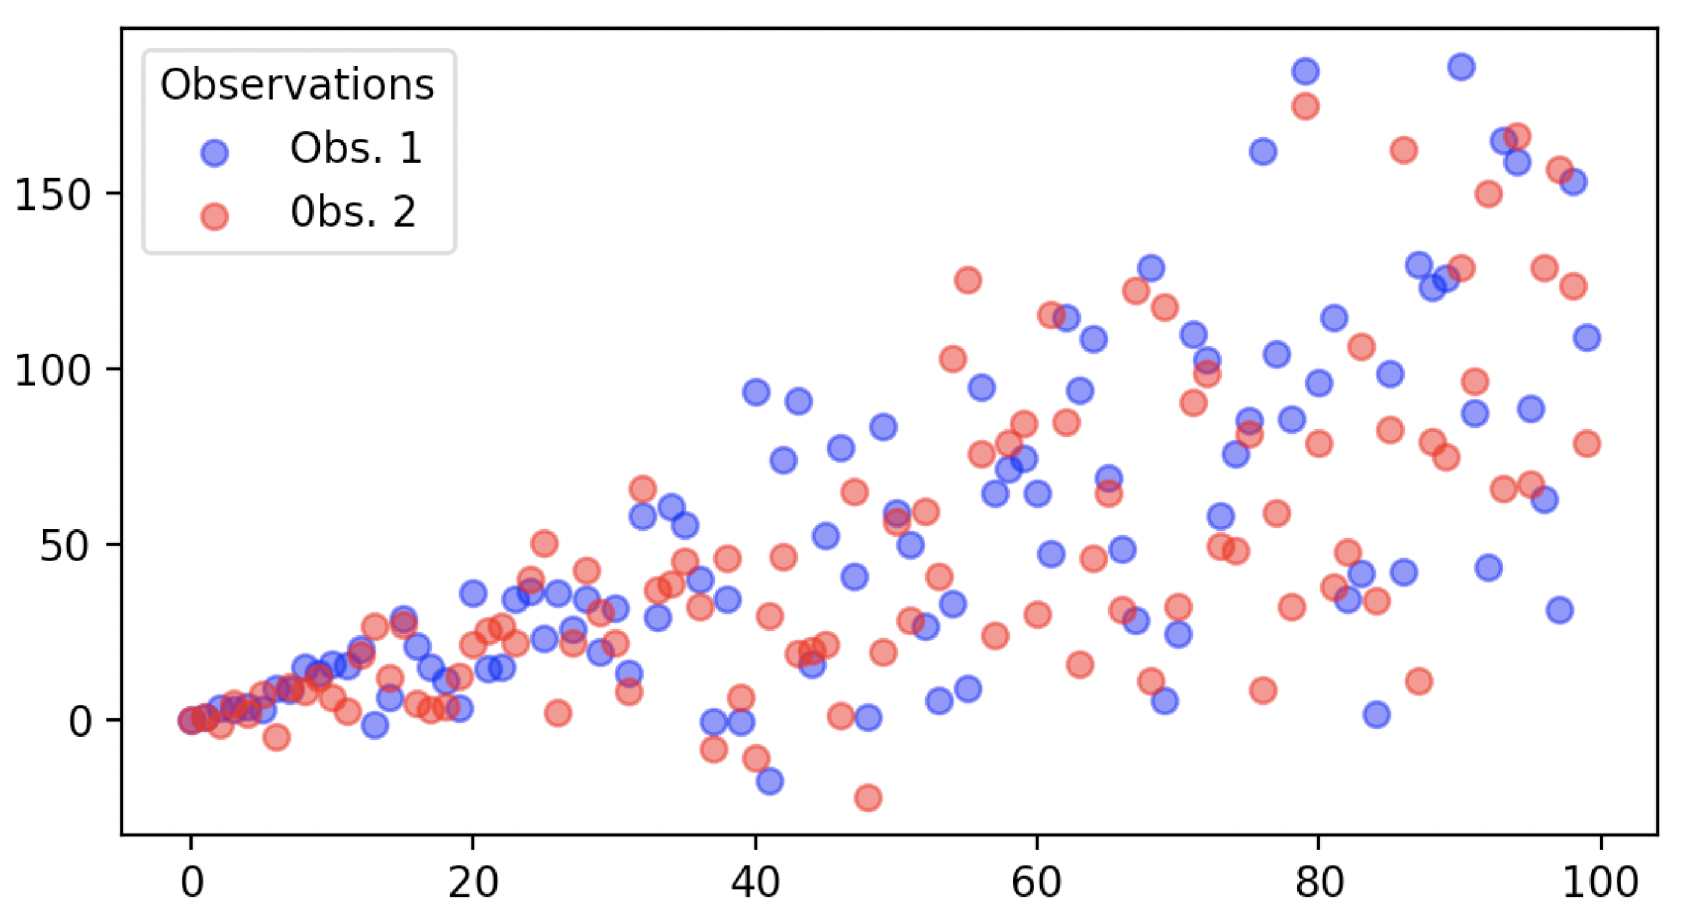
\includegraphics[width=\textwidth]{\dir/two_observations.png}
\caption{}
\label{fig:illustration_random_array}
\end{figure}

\subsection{What happens if we do ERM?}

If we follow standard ERM, then we would estimate $i^*$ with 
%
$$\hat{i} := \argmin_{i \leq n} X'_i + X''_i.$$ 
%
That is, the popular wisdom in statistical learning advocates to estimate $i^*$ with the index where the minimum of $X' + X''$ is. However, this approach fails in probability as $n$ increases. This is because, with high probability, there is some $i > 0$ for which $X'_i + X''_i < X'_0 + X''_0$.

\subsection{What happens if we do ME+PA?}

ME+PA correctly estimates $i^*$ much more often than ERM. To demonstrate this, we set $n = 1000$ and conducted an experiment where we drew at random 1000 pairs $(X', X'')$ of independent observations from $\mathfrak{X}$'s distribution. For each pair, we executed ERM and ME+PA to estimate $i^*$. We counted how often each value $i \leq n$ was chosen as the estimate by each method. Figures~\ref{fig:erm_array} and~\ref{fig:mepa_array} demonstrate that in ~20\% of the cases, ME+PA selects $i^*$ as the estimate, whereas ERM never picks it.

\begin{figure}
\centering
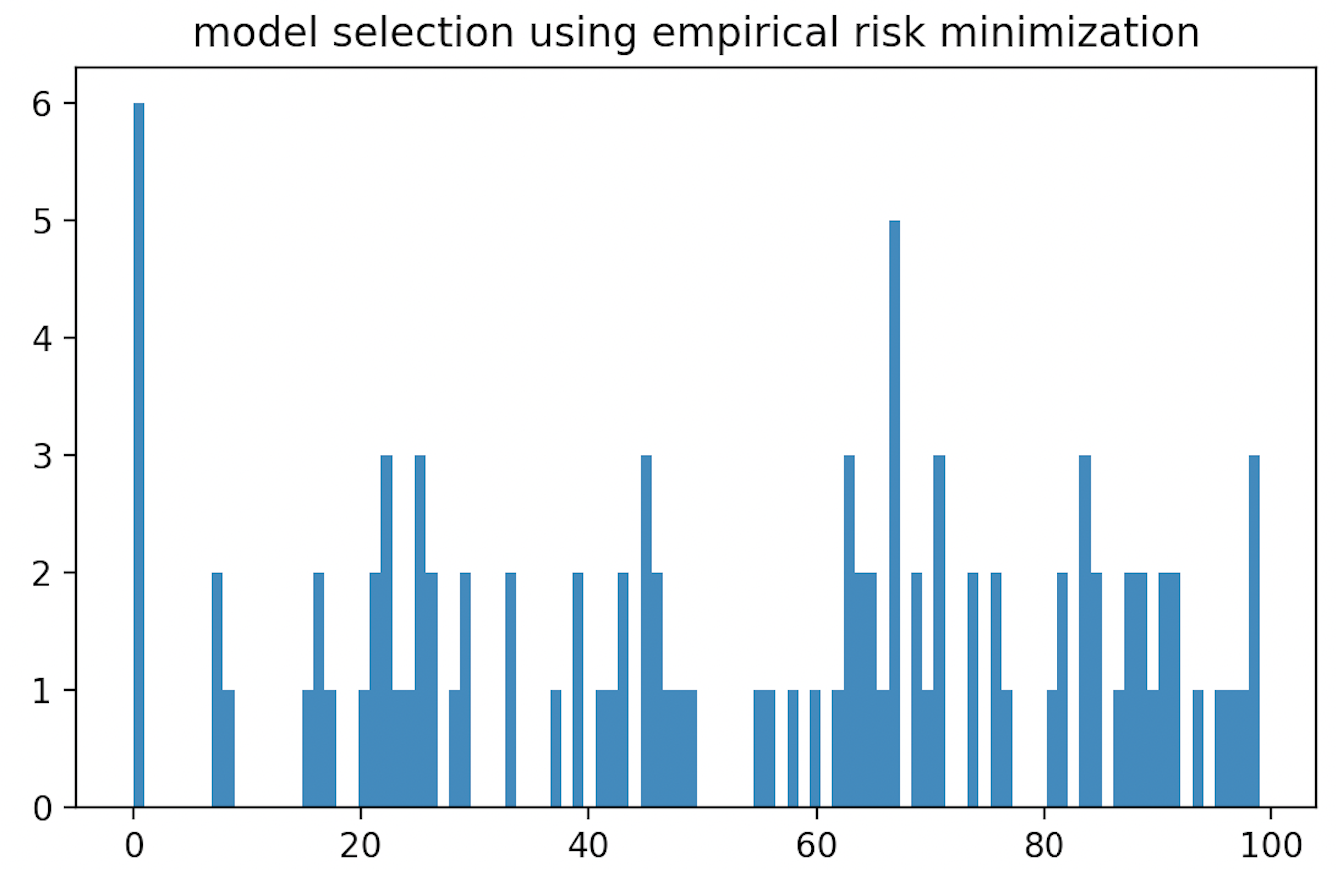
\includegraphics[width=0.8\textwidth]{\dir/erm_array.png}
\caption{Histogram counting how often each estimate in \{0, \ldots, 999\} was picked by ERM as the estimate for $i^*$ across 1000 trials. Observe that ERM never picked the correct estimate.}
\label{fig:erm_array}
\end{figure}

\begin{figure}
\centering
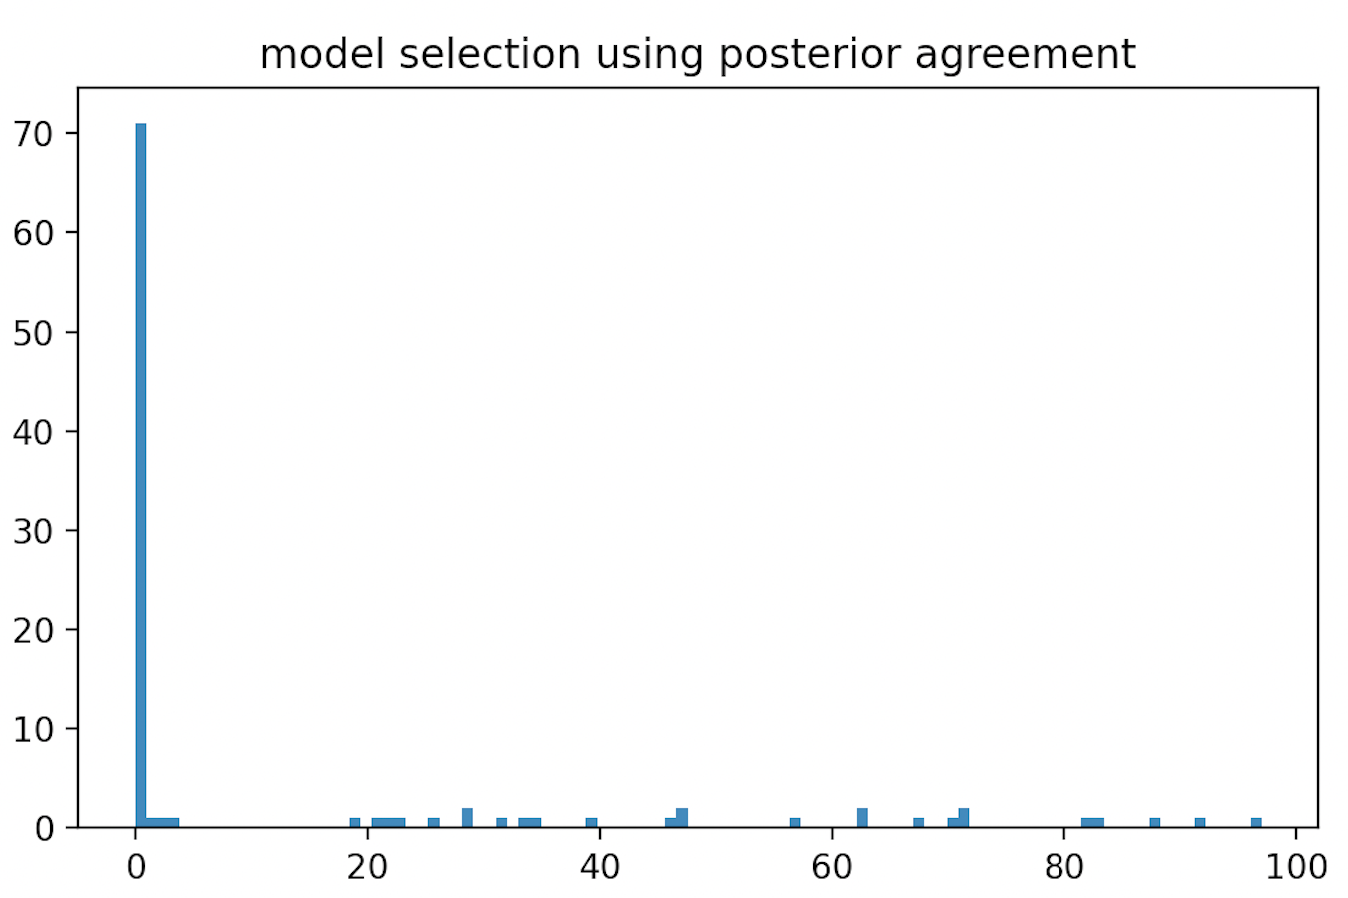
\includegraphics[width=0.8\textwidth]{\dir/mepa_array.png}
\caption{Histogram counting how often each estimate in \{0, \ldots, 999\} was picked by ME+PA as the estimate for $i^*$ across 1000 trials. In contrast to ERM, ME+PA picks the correct estimate around 20\% of the time.}
\label{fig:mepa_array}
\end{figure}

\subsection{Application of ME+PA}

We now illustrate the steps to apply ME+PA to this problem.

First, the hypothesis class is $\mathcal{C} = \{0, \ldots, n-1\}$ and the set $\mathcal{X}$ is $\mathbb{R}^n$.

Let $X \in \mathcal{X}$ be an observation. The cost function is $R(c, X) = X_c$. The Gibbs distribution is given by $p(c \mid X) \propto \exp\left(-1/T X_c\right)$. For the two given observations $X'$ and $X''$, a combined Gibbs distribution is $p(c \mid X', X'') \propto \exp\left(-1/T \left(X'_c + X''_c\right)\right)$.

We now need to define a value for $T$. We guess a set of candidate values and, for each of them, we compute the posterior agreement kernel $\kappa(X', X'')$. We then pick the value that yielded the maximum posterior agreement kernel. Finally, we just choose the $\hat{c}$ with largest $p(\hat{c} \mid X', X'')$.

\section{Maximum entropy}
\label{sec:max_entropy}

In this section, we explain the rationale behind the Gibbs distribution. Remember that for an observation $X$, we want to have a distribution $p(\cdot \mid X)$ such that, for $c \in \mathcal{C}$, $p(c \mid X)$ measures how much we believe that $c$ is the right model for $X$. The base for that measure is the cost $R(c, X)$. The lower this cost is, the more we believe that $c$ is the right model for $X$. We can therefore elicit the following requirement:

\begin{requirement}

For any $X \in \mathcal{X}$ and any $c_1, c_2 \in \mathcal{C}$, $R(c_1, X) \leq R(c_2, X)\Leftrightarrow P(c_1 \mid X) \leq P(c_2 \mid X)$.

\end{requirement}

There are too many distributions that fulfil this requirement. To narrow the set of candidate distributions, we follow the \emph{maximum entropy principle}~\cite{jaynes1957information, jaynes1957information2}. 

The maximum entropy principle states that when choosing between two distributions that equally fulfil some criteria, choose the one with the highest entropy. This is equivalent to choosing the distribution that is ``closest'' to the uniform distribution with respect to the Kullback-Leibler divergence. By aiming for the ``most uniform'' distribution, we aim for a distribution that does not show arbitrary preferences for one model over the other. The distribution should only show preferences based on the cost function.

\begin{requirement}
$P(\cdot \mid X)$ shall have maximum entropy.
\end{requirement}

Finally, we add some regularity requirements.

\begin{requirement}
$P(\cdot \mid X)$ is a regular distribution. That is, $P(c \mid X) \geq 0$, for any $c \in \mathcal{C}$, $\sum_{c \in \mathcal{C}} P(c \mid X) = 1$, and $\mathbb{E}_{C \sim p(\cdot \mid X)}[R(C, X)] < \infty$.
\end{requirement}

These requirements define a constrained optimization problem
%
\begin{align}
\max_{p} \quad& H[p]\label{eq:max_ent_gibbs}\\
s.t. \quad& p(c_1) \leq p(c_2), \text{ for any $c_1, c_2 \in \mathcal{C}$ with $R(c_1, X) \leq R(c_2, X)$,}\label{req:max_ent_mono}\\
& p(c) \geq 0, \text{ for $c \in \mathcal{C}$,}\label{req:max_ent_nonneg}\\
& \sum_{c \in C} p(c) = 1, \label{req:max_ent_massone}\\
& \mathbb{E}_{C \sim p}[R(C, X)] = \mu. \label{req:max_ent_fixexp}
\end{align}
%
Here, $\mu$ is a hyper-parameter ensuring that the expectation is finite. We will later see that its exact value is not important and can be chosen using the posterior agreement principle.

We solve this problem by using Lagrange multipliers, forgetting about the inequality constraints, and then showing that the solution happens to fulfil those inequality constraints. The Lagrangian in this case is
%
\begin{equation}
\mathcal{L}(p, \lambda_1, \lambda_2) = H[p] + \lambda_1 \left( 1- \sum_{c \in \mathcal{C}} p(c)\right) + \lambda_2 \left(\mathbb{E}_{C \sim p}[R(C, X)] - \mu\right).
\label{eq:max_ent_lag}
\end{equation}
%
Therefore, for $c \in \mathcal{C}$,
%
\begin{equation}
\frac{\partial \mathcal{L}}{\partial p(c)} = -1 -\log p(c) + \lambda_1 + \lambda_2 R(c, X).
\end{equation}
%
Setting this expression equal to zero and solving for $p(c)$, while using the constraint that $\sum_c p(c) = 1$, yields that
%
\begin{equation}
p(c) \propto \exp(-\lambda_2 R(c, X)).
\end{equation}

Observe that $p(\cdot)$ already fulfils the constraint~(\ref{req:max_ent_nonneg}). If we enforce the constraint~(\ref{req:max_ent_mono}), then $\lambda_2$ must be non-negative. Furthermore, if $\lambda_2 = 0$, which is the case when $\mu = 1/ \left|\mathcal{C}\right| \sum_c R(c, X)$, then $p(\cdot)$ is the uniform distribution over $\mathcal{C}$, which is not interesting for us as $p(\cdot)$ does not discriminate the different models in $\mathcal{C}$ in this case. We can therefore agree that $\lambda_2 > 0$. To make this distribution look more like the Gibbs distribution used in statistical physics to model particle systems, we define $T := 1 / \lambda_2$. Hence, the solution of the constrained optimization problem is
%
\begin{equation}
p(c) \propto \exp\left(-\frac{1}{T} R(c, X)\right), \text{ for some $T > 0$.}
\label{eq:the_max_ent_dist}
\end{equation}

We refrain from computing the exact value for $T$ as it is analytically very difficult and unnecessary. The value of $T$ is defined by $\mu$, which is a hyper-parameter. Hence, we just leave $T$ as another hyper-parameter. $T$ can also be seen as a concentration hyper-parameter, defining how concentrated $p(\cdot)$ is around the global minima of $R(c, X)$. To see this, we have the following exercise.

\begin{exercise} Prove that
%
\begin{equation}
\lim_{T \to \infty} p(c) = \frac{1}{\left|\mathcal{C}\right|}. 
\end{equation}

\begin{equation}
\lim_{T \to 0} p(c) = \begin{cases}
a & \text{if $c \in \argmin_{c \in \mathcal{C}} R(c, X)$}\\
0 & \text{otherwise.}
\end{cases}
\end{equation}
%
Here, $a$ is a constant value.
\label{ex:gibbs_dist_extreme_temps}
\end{exercise}

Observe that $p$ is unique. Any other $p'$ that solves the constrained problem must also have the form given by Equation~(\ref{eq:the_max_ent_dist}). Hence, the difference between $p'$ and $p$ must be in their corresponding values for $T$, but observe that a change in $T$ induces a change in $\mathbb{E}_{C}[R(C, X)]$. As a result, it is impossible that $p \neq p'$ if both happen to solve the constrained optimization problem and have $\mathbb{E}_{C\sim p}[R(C, X)] = \mathbb{E}_{C\sim p'}[R(C, X)] = \mu$.
%
%Notice that $\mu$ must be between $\min_{c \in \mathcal{C}} R(c, X)$ and $\max_{c \in \mathcal{C}} R(c, X)$. When $\mu = \min_{c \in \mathcal{C}}$, if it exists, $p$ must be a uniform distribution over the global minima of $R(\cdot, X)$. Hence, $\lambda_2 = \infty$ in this case. When $\mu = \max_{c \in \mathcal{C}}$, if it exists, $p$ must be a uniform distribution over the global maxima of $R(\cdot, X)$. Hence, $\lambda_2 = -\infty$ in this case. When $\mu = 1/ \left|\mathcal{C}\right| \sum_c R(c, X)$, one can show that $\lambda_2 = 0$, which makes sense as this results in $p(\cdot)$ being the uniform distribution over $\mathcal{C}$.

The results in this section can be naturally adapted in some cases when $\mathcal{C}$ is not discrete, like $\mathbb{R}^m$. In this case, one of the main challenges is to ensure that the Gibbs distribution has a bounded normalization constant. This is usually satisfied if the cost function goes to $\infty$ fast enough as $\left\|c\right\| \to \infty$.

\begin{exercise}
Let $\mathcal{C} = \mathbb{R}^m$ and $\mathcal{X}$ denote all subsets of pairs $(x, y) \in \mathbb{R}^m \times \mathbb{R}$. Consider the sum-of-squares cost function used for linear regreesion, which is defined for $c \in \mathcal{C}$ and $X \in \mathcal{X}$ as follows:
%
\begin{equation}
R(c, X) = \sum_{(x, y) \in \mathcal{X}} \left(y - c^\top x\right)^2 + \lambda \left\|c\right\|^2.
\end{equation}
%
Demonstrate that the solution to the constrained optimization problem given by Equations~\ref{eq:max_ent_gibbs}---\ref{req:max_ent_fixexp} is given by
%
$$p(\cdot \mid X) \propto \exp\left(-\frac{1}{T}R(c, X)\right), \quad \text{with $T > 0$}.$$
%
\end{exercise}

Observe that without the regularization term $\lambda \left\|c\right\|^2$, it would not be possible to satisfy all the constraints.

\section{Relation between the holdout and ME+PA}

Many training algorithms require hyper-parameters to define the hypothesis class $\mathcal{C}$. A common technique to select those hyper-parameters is \emph{the hold-out}. 

In the hold-out, we draw two samples $X'$ and $X''$, usually called the \emph{training sample} and the \emph{testing sample} respectively. Models are trained in $X'$ and then evaluated in $X''$. A natural evaluation metric is \emph{the out-of-sample error}:
%
\begin{align}
\mathbb{E}_{C | X'}\left[R(C, X'')\right] &= \mathbb{E}_{C | X'}\left[- T \log p(C \mid X'')\right]\\ 
&\propto - \int p(c \mid X') \log p(c \mid X'') \, dc.
\end{align}
%
Here, $p(C \mid X')$ and $p(C \mid X'')$ are Gibbs distributions induced by $R$ and some temperature $T$.

The hold-out advocates to select the hyper-parameter that minimizes this error.

In contrast, posterior agreement advocates to select the hyper-parameter that maximizes the posterior agreement kernel induced by $R$ and some temperature $T$:
%
\begin{equation}
\mathbb{E}_{C | X'}\left[p(C \mid X'')\right].
\end{equation}

We argue here that the posterior agreement kernel is less sensitive to noise than the out-of-sample error. To see this suppose that $X' = X + \Delta'$ and $X'' = X + \Delta''$, where $X \in \mathbb{R}^m$ and that $\Delta', \Delta''$ are distributed according to a Gaussian. Furthermore, we assume that $\left\|\Delta'\right\| < 1$ and $\left\|\Delta''\right\| < 1$. 

\begin{exercise} Show that
%
\begin{equation}
\mathbb{E}_{C | X'}[R(C, X'')] = \mathbb{E}_{C | X}[R(C, X)] + O(\left\|\Delta\right\|) \text{ and}
\end{equation}
%
\begin{equation}
\mathbb{E}_{C | X'}[p(C \mid X'')] = \mathbb{E}_{C | X}[R(C, X)] + O(\left\|\Delta\right\|^2).
\end{equation}
%
Use the following second-order Taylor approximation:
%
\begin{equation}
p(C \mid X') = p(C \mid X) + \left(\nabla_{X}p(C\mid X)\right)^\top \Delta + O(\left\|\Delta\right\|^2).
\end{equation}
%
\end{exercise}
%
% of where we score candidates for the hyper-parameter values with the \emph{validation error}

%

%The expectation is over a \emph{validation set} of examples, which in our framework is just another observation from our phenomenon. Since we do not have access to the 

%A popular model validation technique is cross validation. In this technique we a model $c \in \mathcal{C}$

%

%\todo{Complete this proof.}

\section{Informal justification and motivation}
\label{sec:inf_justification}

\todo{Prepare intuitive explanation}

\todo{Demonstrate the entire workflow of ME+PA for clustering.}

